\documentclass[a4paper]{article}
\usepackage{listings}
\usepackage{float}
\begin{document}
\title{WSNBroadcast, a broadcast algorithm}
\author{Vassilis Vassiliadis\\vasiliad@inf.uth.gr}
\maketitle

\section{Usage}

My broadcast algorithm is essentially the implementation of the WSNBroadcastC interface which is presented at Listing \ref{wsnbroadcastc}.

\begin{lstlisting}[float=h, caption=WSNBroadcastC.nc Interface., label=wsnbroadcastc]
interface WSNBroadcastC {
  command error_t send(void *data, uint8_t len);
  event   void    receive(void *data, uint8_t len, uint16_t source,
      uint16_t last_hop, uint8_t hops);
}
\end{lstlisting}

When an applicaton uses the WSNBroadcastC interface it uses the send(...) command
to broadcast a message of size len. When a node receives a packet the following information
is passed on to the application.

\begin{itemize}
\item The packet payload.
\item The packet size.
\item The number of times the packet was broadcasted till it reached the current node (number of hops).
\item The address of the last node which broadcasted the packet.
\end{itemize}

Additionally the implementation allows for usage by different applications present on the same node in the same way
that the Active Messages enable the developer to use different streams of communication by specifying an id
during the wiring of the components.


\section{Implementation Details}
\subsection*{Assigning unique IDs to each packet}

Each broadcast message is tagged with an id. The id is the concatenation of the source node's address 
(2 bytes) and a sequence number which is increased each time the node decides to broadcast a packet (Source:sequence).


\subsection*{Fresh and stale packets }
When a node receives a packet it checks whether or not it is considered a "fresh" one. A fresh packet is one for which
one of the following applies:

\begin{itemize}
\item No previous packet from the source node exists in the receiving nodes database.
\item A packet with the same originating node exists in the receiving nodes database whose ID is lower.
\end{itemize}

When a newly received packet is deemed fresh then if a previous broadcast id is present in the ID queue
it is replaced by the new one. In the event that there is no information regarding the originating source node,
then a new entry is placed in the ID queue, if the event queue is full then the oldest entry is replaced
by the new one.

The notion behind this choice is that since packets originating from the same node have sequential ids
if a packet which was just received is not "fresh" in the scope of the ID queue then it is dropped. This
way cycles in the network do not result in an infinite propagation of the same packets.

\subsection*{Message Buffer}

Active Messages do not implement a message queue, when the network is under strain (for example multiple
nodes attempt to broadcast a packet) a node may require a storage space in order to store the messages
until they are broadcasted. In order to address this issue I implemented a cyclical buffer to store
all packets that are considered fresh and will eventually be broadcasted to the network.

When the buffer is full any messages received from the network will be dropped, however if a node attempts
to send a packet of its own it will overwrite the last packet in the buffer. The reasoning behind this choice
is that a message received over the network will probably be received from another node as well.

\subsection{Actions that are performed when a message is received}

The algorithm is best explained with a visual representation.

\begin{figure}[h]
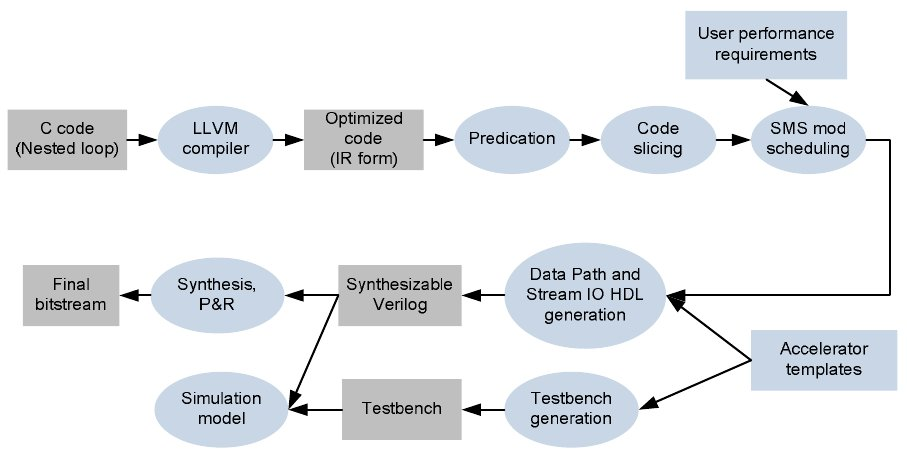
\includegraphics[width=0.7\linewidth]{figures/sopencl_generation.jpeg}
\end{figure}

\section{Metrics}

Using a tool that generate topologies, multiple experiments were performed in order to assess the performance
of the protocol. The topologies that were used consisted of 100 nodes each one having 2 to 5 immediate neighbors.
The nodes would issue 1 broadcast packet every 15 seconds. In tables 1, 2, 3, and 4 the
average packets received are shown for 5, 10, 15, and 20 available slots in the message queue respectively.

\begin{table}[H]
\centering
\begin{tabular}{|c|c|c|}
\hline
Received&	Duplicates& 	ID Buffer Size \\
\hline
59&	2	&	5 \\
\hline
52&	2	&	10 \\
\hline
59 &	2	&	15 \\
\hline
64&	1&	20 \\
\hline
\end{tabular}
\label{f1}
\caption{Message Queue size: 5}
\end{table}

\begin{table}[H]
\centering
\begin{tabular}{|c|c|c|}
\hline
Received&	Duplicates& 	ID Buffer Size \\
\hline

62 &	2	 &	5 \\
\hline

71 &	2	&	10 \\
\hline

75 &	10 &	15 \\
\hline

78 &	10 &	20 \\
\hline
\end{tabular}
\label{f2}
\caption{Message Queue size: 10}
\end{table}

\begin{table}[H]
\centering
\begin{tabular}{|c|c|c|}
\hline
Received&	Duplicates& 	ID Buffer Size \\
\hline
71&2&5 \\
\hline
75&2&10 \\
\hline
80&2&15 \\
\hline
83&2&20 \\
\hline
\end{tabular}
\label{f3}
\caption{Message Queue size: 15}
\end{table}


\begin{table}[H]
\centering
\begin{tabular}{|c|c|c|}
\hline
Received&	Duplicates& 	ID Buffer Size \\
\hline
74&3&5 \\
\hline
79&2&10 \\
\hline
83&2&15 \\
\hline
84&2&20 \\
\hline
\end{tabular}
\label{f4}
\caption{Message Queue size: 20}
\end{table}

Another experiment was simulated in which 300 nodes broadcasted a packet once every minute, on average each node
received 231 packets out of 299 with 3 additional duplicate messages on average. For this test run I used a
message queue of 30 packets and a buffer which could contain 30 broadcast IDs.

The numbers indicate that the size of the message queue in - this is the storage space in which packages 
are temporarily placed untill its time for them to be broadcasted - plays a major role in the performance
of the algorithm when the network is under heavy pressure.

\end{document}
